\section{Dokumente und ihr Aufbau}

\subsection{Strukturierung}
\begin{frame}
  \frametitle{Strukturierung}
  \begin{itemize}
  \item Große Dateien → unübersichtlich
  \item Aufteilung pro Abschnitt/Kapitel
  \item Einbinden in Hauptdokument:
    \begin{itemize}
    \item \TeX-Style: \texttt{\textbackslash input\{<filename>\}}
    \item \LaTeX-Style: \texttt{\textbackslash include\{<filename>\}}
    \item Bei \texttt{\textbackslash include}:\\
      \texttt{\textbackslash includeonly\{...\}},
      \texttt{\textbackslash excludeonly\{...\}}
    \end{itemize}
  \item Automatisierter Buildprozess\\
    Makefile, latexmk, arara
  \item Guter Editor\\\pause
    Emacs+AUC\TeX+Ref\TeX\\
    (Befehlstemplates, Automatische Compileaufrufe, math. Symbole über
    Menü mit grafischer Vorschau, Preview von Formeln im Editor,
    Referenzmanagement mit Ref\TeX)
  \end{itemize}
\end{frame}

\begin{frame}
  \frametitle{Buildtools}
  \begin{itemize}
  \item Makefile
    \begin{itemize}
    \item typisch für UNIX-Welt
    \item Nicht für \TeX{} entwickelt → oft komplizierte Winkelzüge notwendig
    \end{itemize}
  \item Arara
    (\href{http://ctan.org/pkg/arara}{\texttt{CTAN;//pkg/arara}})
    \begin{itemize}
    \item Java-Tool
    \item Konfiguration über Java
    \end{itemize}
  \item latexmk
    (\href{http://ctan.org/pkg/latexmk}{\texttt{CTAN://pkg/latexmk}})
    \begin{itemize}
    \item Perl-Tool
    \item Code-Überwachung für automatisches Compiling
    \end{itemize}
  \end{itemize}
\end{frame}

\subsection{Bibliographien}
\begin{frame}
  \frametitle{Bibliographien}
  \begin{itemize}
  \item Früher: \hologo{BibTeX}
  \item Heute: \alert{\textsc{Bib}\LaTeX}
    \begin{itemize}
    \item Unicodefähig
    \item Viele Zitierstile
    \item Einfache Programmierung
    \item Backend \texttt{biber}: Volle Unicodeunterstützung
    \item \href{http://ctan.org/pkg/biblatex}{\texttt{CTAN://pkg/biblatex}}
    \end{itemize}
  \end{itemize}
\end{frame}

\begin{frame}[fragile]
  \frametitle{Bibliographie-Datenbank}
  \examplefile{biblio.bib}
  \lstinputlisting[firstline=1,lastline=10]{biblio.bib}
  \begingroup
  \printbibliography[heading=none,keyword=bibexample]
  \endgroup
\end{frame}

\begin{frame}
  \frametitle{Einbinden in Dokumente}
  \examplefile{examples/bibliography/basic.tex}
  \lstinputlisting[language={[LaTeX]TeX}]{examples/bibliography/basic.tex}
\end{frame}

\begin{frame}
  \frametitle{Einbinden in Dokumente (2)}
  Bild über Compileprozess
\end{frame}

\begin{frame}
  \frametitle{Einbinden in Dokumente (3)}
  Ergebnis:
  \fbox{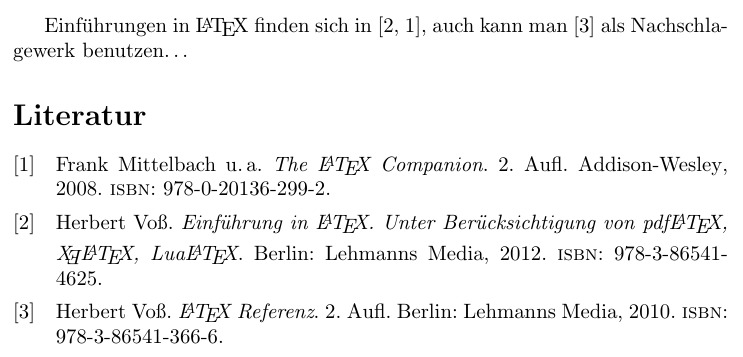
\includegraphics[width=.9\textwidth]{scr-biblatex-simple}}
\end{frame}

\begin{frame}
  \frametitle{Bibliographietypen}
  \begin{itemize}
  \item \texttt{book}\\
    \texttt{author}, \texttt{year}, \texttt{title}
  \item \texttt{online}\\
    \texttt{author/editor}, \texttt{year/date}, \texttt{title},
    \texttt{url}
  \item \texttt{inproceedings}\\
    \texttt{author}, \texttt{editor}, \texttt{title},
    \texttt{booktitle}, \texttt{year/date}
  \item \texttt{article}\\
    \texttt{author}, \texttt{title}, \texttt{journaltitle},
    \texttt{year/date}
  \item \texttt{thesis}\\
    \texttt{author}, \texttt{title}, \texttt{type},
    \texttt{institution}, \texttt{year/date}
  \item Viele weitere Typen und Felder in der Dokumentation
  \end{itemize}
\end{frame}

\begin{frame}
  \frametitle{Zitierstile}
  \begin{itemize}
  \item \texttt{numeric}\\
    Wie im Beispiel ersichtlich (Standardstil)
  \item \texttt{alphabetic}\\
    Alphabetischer Zitierstil: [Voß12], [Mit08]\dots
  \item \texttt{authoryear}\\
    Autor+Jahr Stil: Voß 2012; Mittelbach u.\,a. 2008
  \item Zig weitere (z.\,T. als Erweiterungspakete)\\
    JuraBib, Fußnoten etc.
  \end{itemize}
\end{frame}

\subsection{Indexerstellung}
\begin{frame}
  \frametitle{Indexerstellung}
  
\end{frame}

\subsection{Glossarerstellung}
\begin{frame}
  \frametitle{Glossarerstellung}
  
\end{frame}
%%% Local Variables: 
%%% mode: latex
%%% coding: utf-8
%%% TeX-engine: luatex
%%% TeX-PDF-mode: t
%%% TeX-master: "../pr-ieee-main"
%%% End: 
